\section{Regression method based on SSPA database}
\label{se:correction_SI_method}
In order to improve the accuracy of the roll damping prediction, the SSPA database containing more than 250 roll decay tests with modern ships is used to propose new models. In the following preliminary investigation, two different approaches are used to build such a model for roll damping prediction. The model is assumed to be a function of the same input parameters as the SI-method (see equation \ref{eq:S1-method}). It was found in section \ref{se:overall_comparison} that the $B_e$ coefficient changes a lot with the roll amplitude $\phi_a$ which introduces a challenge to this regression. Three different options to approach this were considered:
\begin{itemize}
    \item Calculate $B_e$ for only one representative value of $\phi_a$.
    \item Split the problem into two regressions, one for $B_1$ and one for $B_2$.
    \item Calculate $B_e$ for a range of $\phi_a$ and include all in the regression.
\end{itemize}
The first option was rejected because that would generate a model that works for one roll amplitude only. The second option was rejected because introducing two regression models was considered unnecessary complex. And it was also suspected that there could be correlations between $B_1$ and $B_2$ so that the two regressions needed to be connected in some way. So the third option was used which means that the $B_e$ used in the regression contains roll amplitudes between 0 and 10 degrees.  

\subsection{New regression model for roll damping}
The first approach assumes that the function can be expressed as a second order polynomial. Some statistical learning method is used to establish the regression model. The input parameters (the features) are first transformed into polynomial features including all possible coupling terms. The best polynomial features are selected using a feature selection algorithm, selecting the k-best features \parencite[]{noauthor_sklearnfeature_selectionselectkbest_nodate} with a linear model for testing the individual effect of each feature \parencite[]{noauthor_sklearnfeature_selectionf_regression_nodate}. 

Cross validation, as described in section \ref{se:cross_validation} below, is used to estimate the accuracy. The optimum number of polynomial features was determined by finding the "k-value" with the highest accuracy in the cross validation. A regression model with 12 polynomial features was found to have the best accuracy when evaluated in this way. The model was determined by fitting the selected regression model to the entire data, giving the following expression:

\begin{equation} \label{eq:polynom_complex}
\begin{aligned} 
 \hat{B_{e}} = - 0.02578 A_{0} V - 0.02705 BK_{B} V + \\ 
 0.008993 BK_{L} V - 0.03191 C_{b} V - 0.2028 OG V + \\ 
 0.003472 V^{2} + \\ 
 0.004234 V \hat{\omega_{0}} - 0.008384 V beam - 0.002591 V phi_{a} + \\ 
 0.05048 V + \\ 
 0.007814 \hat{\omega_{0}}^{2} + \\ 
 0.03882 \hat{\omega_{0}} phi_{a} - 0.001069 \\ 
 \end{aligned}
\end{equation}

All the inputs with length scale ($T$, $B_{KB}, $B_{KL}$, $beam$) are nondimenilaized with $L_{pp}$. $V$ is nondimenionalized using $\sqrt{L_{pp}$. The middsection coefficients $A_0$ and block coefficients $C_b$ are nondimensional. The roll amplitude $\phi_a$ is in radians.


\subsection{Correction of Simplified Ikeda's method}
The second approach uses the SI-method as is, but then applies some corrections to the output damping components. A roll amplitude correction factor was also added. The correction factors was determined by fitting a linear regression model to the roll damping components giving the following expression: 
\begin{equation} \label{eq:polynom_correction}
\hat{B_e} = 1.106 \hat{B_BK_e} - 0.9124 \hat{B_E_e} + 4.282 \hat{B_F_e} + 0.7457 \hat{B_L_e} + 0.1844 \hat{B_W_e} + 0.004999 \phi_{a} - 0.0005097
\end{equation}

The proposed correction factors implies that $\hat{B_{BK}}$ and $\hat{B_{W}}$ should be reduced, $\hat{B_{E}}$ should be made negative and $\hat{B_{L}}$ does not need much correction.

A new semi empirical method to predict roll damping has been developed as an alternative or complement to the simplified Ikeda's method. The method  predicts roll damping as a simple mathematical expression based on main particulars and does not require a hull geometry definition. 
The new method is based on regression of the present roll damping database with some additional components of Ikeda's method. Since the underlying data is collected from roll decay tests, the methods predicts the roll damping at the natural frequency $\omega_0$.  
The regression was conducted on the roll damping database for tests at even keel. 

The roll damping database reveals that the roll damping at zero speed is much lower than the roll damping at speed. The hydrodynamics at zero speed and at speed is very  different \parencite{ikeda_velocity_1979}. These two situations need to be separated so that  the regression is formulated  as a product of two sub models:
\begin{equation} \label{eq:regression_factor_equation}
B_{e hat} = B_{e factor} B_{e hat 0}
\end{equation}

Where $B_{ehat0}$ is a zero speed regression and $B_{efactor}$ is a speed depending regression. A similar approach was used in \parencite{henry_peter_piehl_ship_2016}. Linear regression is  used for the two sub models. 

\subsection{Cross validation}
When constructing a regression model from a data set, over-fitting the data can be a problem. Including too many parameters and/or allowing too high order of the model would give a very good representation of the present roll damping data, but large extrapolation errors when the model is used on other data. Cross validation has been used to "mimic" this situation, where the model should make predictions on "new data", for ships that have not been part of the regression (the training of the model). The model that can make the best prediction on "new data" is considered as the best. The best model has been developed by optimizing the selection of parameters (the features). The regression model was allowed to have features selected from a "gross list" of all available meta data. The linear regression should determine coefficients in a mathematical expression represented as a polynomial up to second order and including coupling terms. The model with a selection of terms that gives the highest score in the cross validation is considered as the best.    

For the cross validation the data was divided into a  training set (80\%) and a testing set (20\%). The selection was made so that all tests with a specific ship model and its loading conditions were all in either the training set or the testing set. Only tests where there were results for both zero speed and speed (for the same loading condition and ship model) were included.

The "gross list" of available features has been chosen as a balance between guessed relevance and to minimize the number of tests that need to be excluded due to missing meta data. 
The number of parameters was also kept to a minimum so that a set of fewer features was selected prior to one with more features if they had similar scoring. As it turned out the developed regression models (equation \ref{eq:polynom_zero} and \ref{eq:polynom_speed}) have no coupling terms or quadratic terms.

The total regression model, consisting of the two sub models, was evaluated using cross validation. 100 random train/test sets were fitted and tested giving an average score: $mean(R^2)=0.68$, with standard deviation $std(R^2)=0.12$.

Figure \ref{fig:B_e_hat0_regression} and \ref{fig:B_e_factor_regression} shows comparisons between the regressions and the corresponding model test data. It can be noted that the speed factor can be up to 3.5 so that the roll damping at speed is 3.5 times larger than the corresponding roll damping at zero speed. The regressed sub models are shown in equation \ref{eq:polynom_zero} and \ref{eq:polynom_speed}. The non-dimensional damping due to hull lift $B_{LHAT}$, from the Ikeda method, is one of the parameters in the speed dependency equation \ref{eq:polynom_speed}. A comparison for the total regression model (equation \ref{eq:regression_factor_equation}) is shown in figure \ref{fig:B_e_factor_regression_total}, where it can be noticed that the error does not have the same ship draught dependence as the simplified method has. 

\begin{equation} \label{eq:polynom_zero}
B_{e hat} = - 0.0136052800165908 A_{0} + 0.759326775676605 BK_{B} + 0.0725876320147426 GM - 0.0303297720484823 T + 0.00126493893040265 \omega_{0 hat} + 0.0143189616219315
\end{equation}

\begin{equation} \label{eq:polynom_speed}
B_{e factor} = 84.1 B_{L HAT} + 3.64 V + 0.468
\end{equation}

{\footnotesize \underline{Note}: All input parameters are normalized using Froude scaling with $L_{pp}$ as scale factor. $\omega_{0hat}$ is non-dimensional according to \parencite{himeno_prediction_1981}.} 

\begin{figure}[H]
\centering
\begin{minipage}{.5\textwidth}
  \centering
  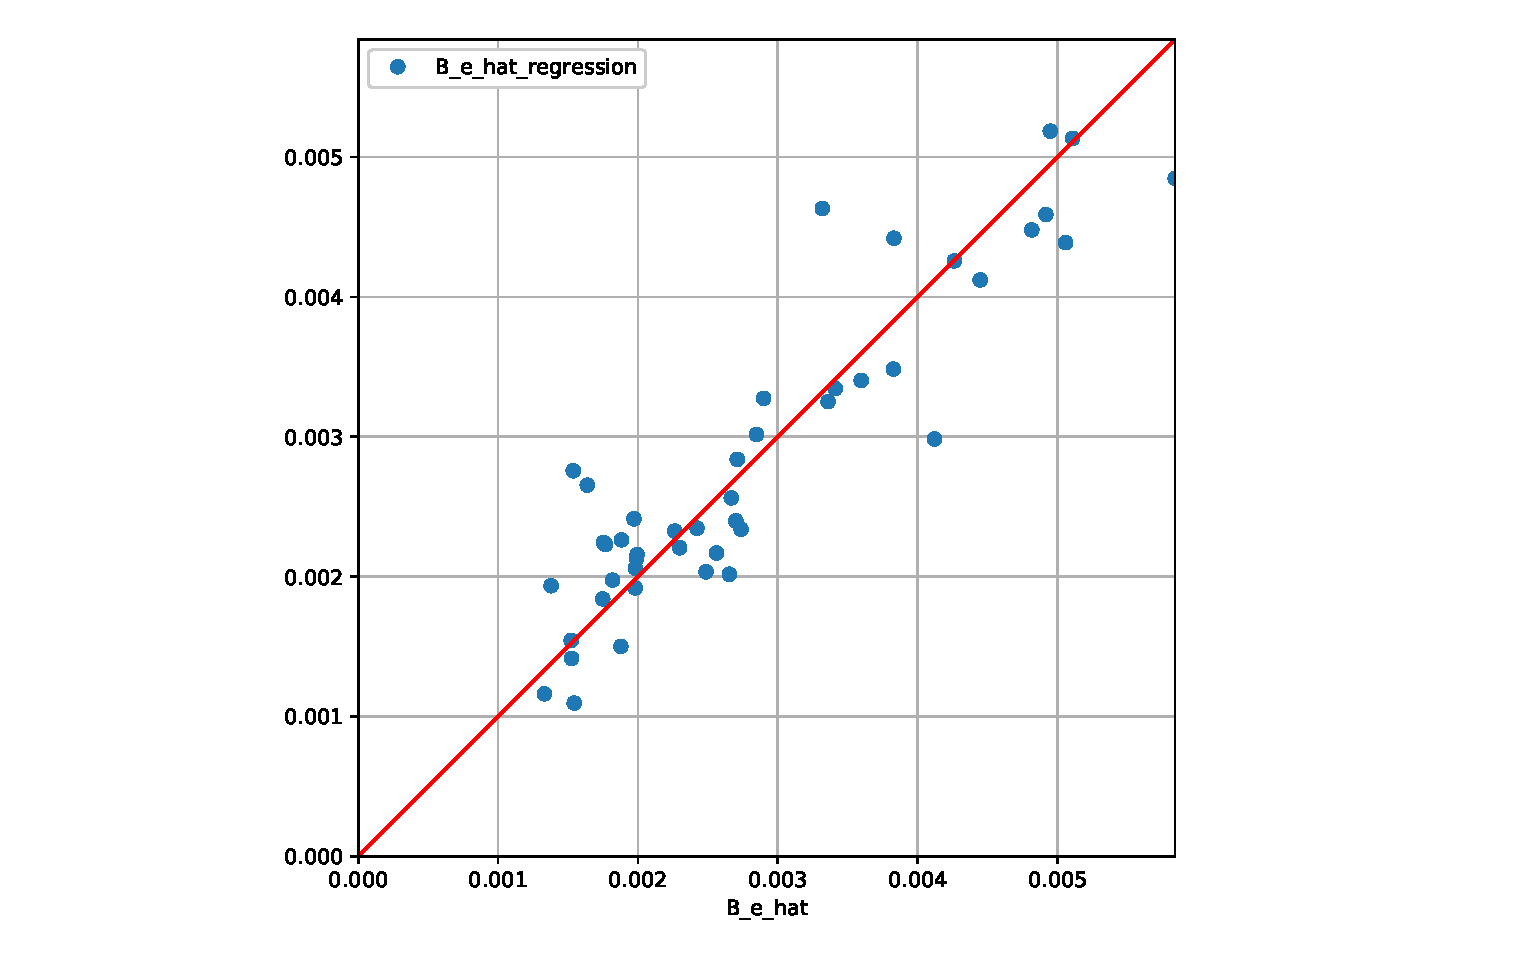
\includegraphics[width=\columnwidth]{figures/B_e_hat0_regression.eps}
    \caption{Comparison between predictions with the zero speed model and the damping at zero speed from the database}
    \label{fig:B_e_hat0_regression}
\end{minipage}%
\begin{minipage}{.5\textwidth}
  \centering
 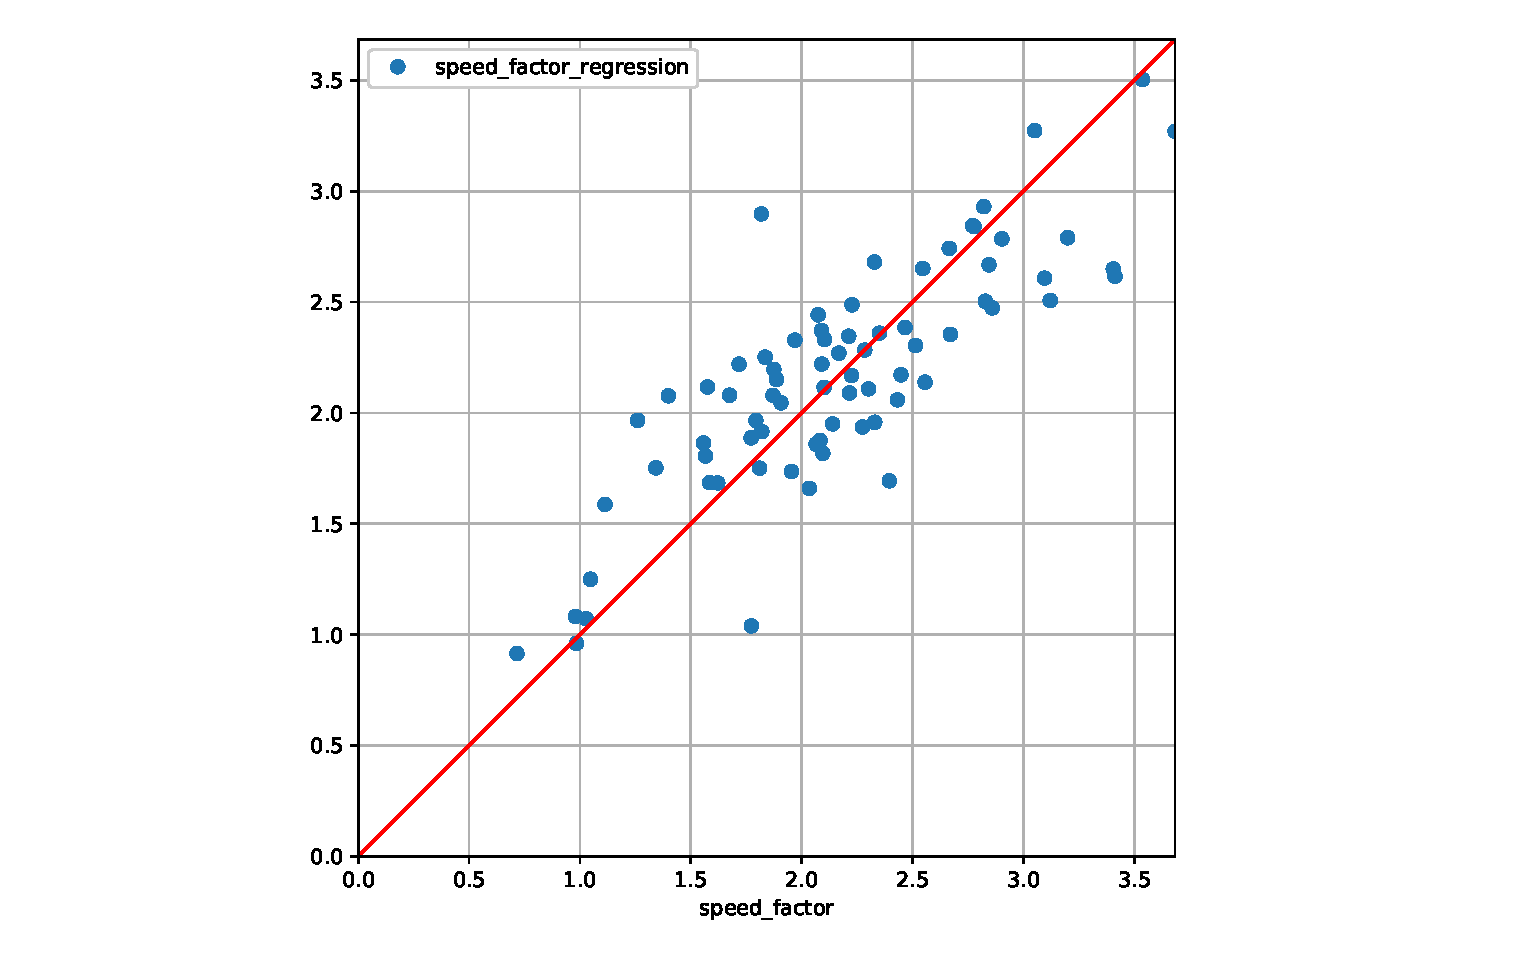
\includegraphics[width=\columnwidth]{figures/B_e_factor_regression.eps}
    \caption{Speed dependency regression}
    \label{fig:B_e_factor_regression}
\end{minipage}
\end{figure}


\begin{figure}[H]
    \centering
    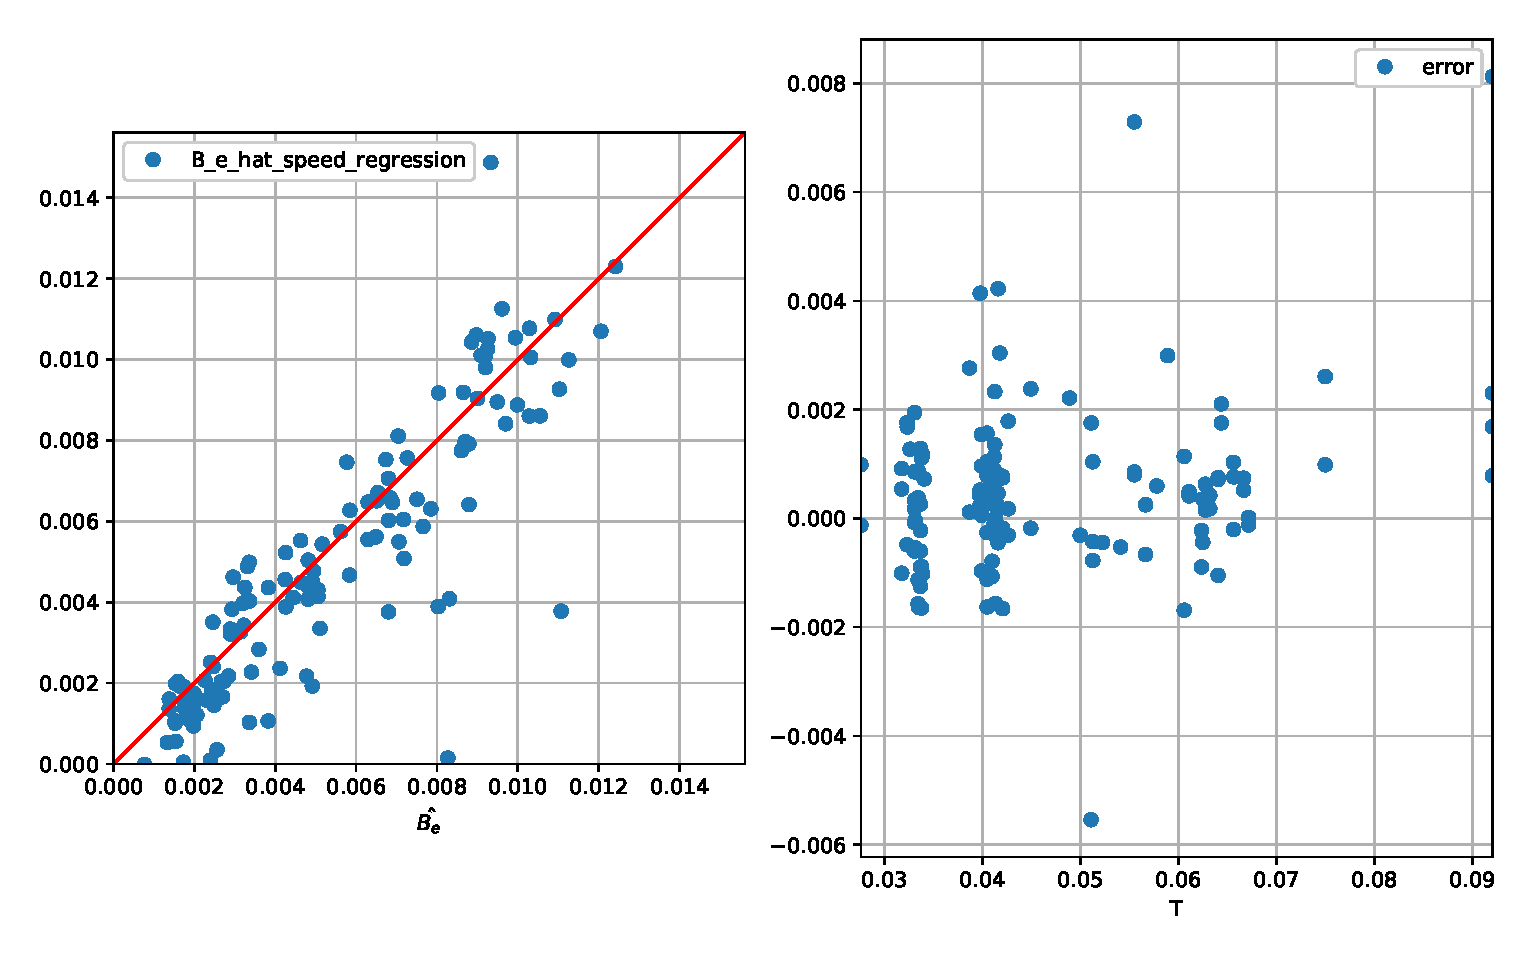
\includegraphics[width=\columnwidth]{figures/B_e_factor_regression_total.eps}
    \caption{Total regression}
    \label{fig:B_e_factor_regression_total}
\end{figure}
